\documentclass{university}

\course{هوش مصنوعی}
\subject{سوالات نظری مینی پروژه دوم}
\professor{دکتر رهبان}

\begin{document}

\setupdocument

\section{}
\subsection{}
غلط، همانطور که در کلاس مطرح شد، الگوریتم به ازای 
\lr{$\epsilon$} 
به اندازه کافی کوچک همگرا می‌شود. با نوشتن بسط تیلور این قضیه اثبات می‌شود. 

\subsection{}
درست، چون مشتق در آن نقطه صفر می‌شود، الگوریتم در همان نقطه متوقف می‌شود. 

\subsection{}
غلط، ممکن است تابع محدب نباشد ولی با شروع از یک نقطه مناسب الگوریتم به 
\lr{$x^*$} 
همگرا شود. شرط دو طرفه نیست. 

\subsection{}
درست، چون الگوریتم به ازای این تابع همگرا می‌شود،  
\lr{$w \neq 0$} 
است و به به یک تابع درجه دو می‌رسیم. میدانیم تابع درجه دو به صورت سهمی رو به بالا یا پایئین است. 
به دلیل همگرایی الگوریتم به ازای این تابع، نتیجه می‌گیریم تابع رو به بالا است. پس تابع 
محدب است و یک مینیمم محلی دارد که همان مینیمم سراسری است. 

\section{}
\subsection{}
میدانیم اگر گراف قیود به شکل درخت باشد، اگر از ترتیب 
\lr{topological sort} 
برای مقداردهی استفاده کنیم، نیاز به 
\lr{backtrack} 
نخواهیم داشت. 
\footnote{این قضیه در کلاس مطرح شده است}
پس ترتیب مورد نظر ‌می‌تواند 
\lr{C-A-B-D-E-F} 
و
\lr{B-C-D-A-E-F} 
باشد. 

\subsection{}
تلاش می‌کنیم با حذف دو گره (چون حداکثر دو بار بک‌ترک داریم) گراف را تبدیل به گراف بدون دور کنیم. 
چون می‌دانیم که اگر گراف بدون دور باشد، بدون بک‌ترک قابل حل است. در این صورت حداکثر دو 
بک‌ترک به ازای تخصیص دو گره حذف شده 
(\lr{cutset})
خواهیم داشت. 

چون دو گره حذف شده را اول مقدار می‌دهیم، بررسی می‌کنیم آیا با حذف دو گره ابتدای ترتیب‌های داده شده از گراف، 
به یک گراف بدون دور می‌رسیم یا نه. 

با توجه به گراف‌های به دست آمده در شکل 
\ref{fig:cutset} 
تنها ترتیب 
\lr{F-C-A-H-E-B-D-G}
مطلوب است. 

\begin{figure}
    \centering
    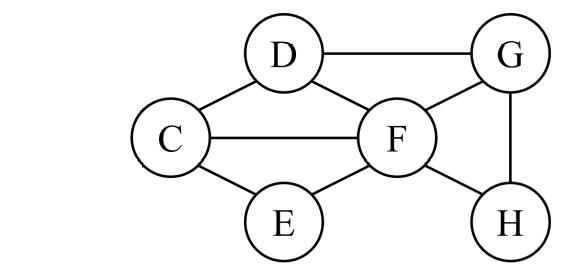
\includegraphics[width=0.5\textwidth]{./assets/2-2-1.png}
    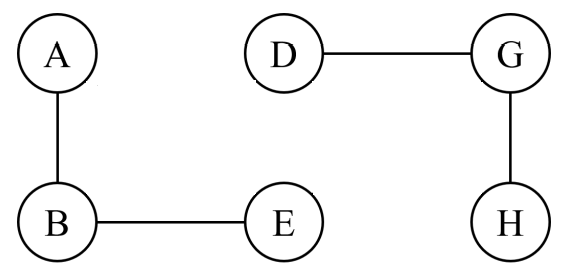
\includegraphics[width=0.5\textwidth]{./assets/2-2-2.png}
    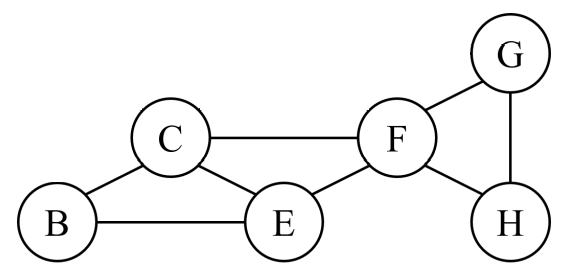
\includegraphics[width=0.5\textwidth]{./assets/2-2-3.png}
    \caption{گراف‌های حاصل با حذف دو گره ابتدایی ترتیب‌ها}
    \label{fig:cutset}
\end{figure}

\subsection{}
از آنجایی که در جفت این مسائل با ساختار بدون دور مسئله را حل می‌کنیم، ترتیب انتخاب متغیرها تاثیری ندارد 
پس 
\lr{MRV} 
بی تاثیر است.

از طرف دیگر چون نمیدانیم تعداد کل جواب‌ها چند تا است، باید تمام مقادیر را امتحان کنیم پس 
\lr{LCV} 
هم تاثیری ندارد.

\section{}

\textbf{(برگ‌های از چپ به راست شماره‌گذاری شده‌اند)} \\

در صورتی که مقدار برگ سوم از ماکس دو برگ اول بیشتر شود راست‌ترین برگ ممکن است هرس شود. یک مثال از هرس شدن آن در شکل 
\ref{fig:prone}
آمده است. 

\begin{figure}[!htbp]
    \centering
    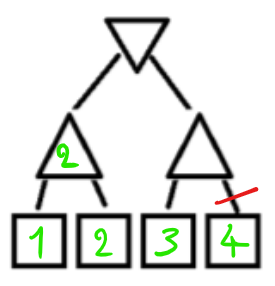
\includegraphics[width=0.3\textwidth]{assets/3.png}
    \caption{مثال هرس شدن}
    \label{fig:prone}
\end{figure}

\subsection{}
همانطور که در کلاس هم گفته شد، هرس کردن در 
\lr{expectimax} 
تنها وقتی ممکن است که حد بالا یا پائین برای دامنه متغیرها داشته باشیم که در اینجا نداریم. 
پس هیچ یک از برگ‌ها هرس نمی‌شوند.

\subsection{}
برای قسمت اول، علاوه بر حالت ذکر شده، زمانی که برگ‌های اول و دوم صفر باشند، کل شاخه سمت راست گره مینیمم هرس می‌شود. 
همچنین اگر چپ‌ترین برگ مقدار 9 را داشته باشد، برگ دوم هرس می‌شود. این حالت برای وقتی برگ سوم 9 است، 
برای برگ چهارم نیز رخ می‌دهد.

برای قسمت دوم اگر میانگین برگ سوم و 0 از میانگین برگ یک و دو بیشتر باشد، برگ چهارم هرس می‌شود. 
همچنین اگر برگ یک و دو صفر باشند، کل شاخه سمت راست گره مینیمم هرس می‌شود.

\end{document}